\documentclass[11pt, a4paper]{article}
\usepackage[utf8]{inputenc}
\usepackage[T1]{fontenc}
\usepackage[spanish]{babel}
\usepackage{geometry}
\usepackage{graphicx}
\usepackage{booktabs}
\usepackage{multirow}
\usepackage{hyperref}
\usepackage{xcolor}
\usepackage{fancyhdr}

\geometry{left=2.5cm, right=2.5cm, top=3cm, bottom=3cm}

\title{\textbf{Entrega 4: Análisis Geoespacial y Estadísticas de Techos por Municipio PDET} \\
\large Flujo Reproducible de Validación y Visualización}
\author{Samuel Emperador Contreras}
\date{Noviembre 2026}

\pagestyle{fancy}
\fancyhf{}
\rhead{Entrega 4}
\lhead{Análisis de Techos PDET}
\cfoot{\thepage}

\begin{document}

\maketitle

\section*{Resumen Ejecutivo}

Este informe presenta un análisis reproducible de edificaciones y área de techos aprovechables en los 170 municipios PDET de Colombia, utilizando Microsoft Global ML Building Footprints (versión 2026-02-03). El flujo automatizado compila datos de múltiples fuentes, genera visualizaciones geoespaciales, y produce tablas de municipios destacados para facilitar la comparación y validación de resultados.

\textbf{Resultados Principales:}
\begin{itemize}
    \item \textbf{170 municipios PDET} con geometrías validadas
    \item \textbf{1.720.535 edificaciones} detectadas por Microsoft
    \item \textbf{220,27 km²} de área total de techos
    \item \textbf{Correlación Spearman 0,904} con Google Building Footprints (en municipios con cobertura completa)
    \item \textbf{15 municipios} con cobertura insuficiente de Google (marcados en este informe)
\end{itemize}

\newpage
\tableofcontents
\newpage

\section{Reproducibilidad y Metodología}

\subsection{Fuentes de Datos}

\begin{itemize}
    \item \textbf{Microsoft Global ML Building Footprints:} Versión 2026-02-03, Licencia ODbL 1.0, accedida el 13 de noviembre de 2026.
    \item \textbf{Capas Municipales:} MGN2025 del DANE (Dirección Nacional de Estadística), 170 municipios PDET.
    \item \textbf{EDA de Entrega 3:} Comparativa con Google Building Footprints (\textit{outputs/eda/eda\_buildings\_summary.json}).
\end{itemize}

\subsection{Pipeline de Procesamiento}

El análisis se ejecuta mediante cuatro scripts de Python que leen datos automáticamente sin transcripción manual:

\begin{enumerate}
    \item \textbf{scripts/07\_entrega4\_analysis.py:} Lee \textit{outputs/rooftop\_stats\_ms.csv} y \textit{outputs/eda/eda\_buildings\_summary.json}. Agrega estadísticas por municipio y subregión. Genera \textit{outputs/entrega4\_analysis\_summary.json}.

    \item \textbf{scripts/08\_entrega4\_visualizations.py:} Carga \textit{data/processed/municipalities.geojsonl} con geopandas. Une con estadísticas por código municipal. Genera mapas coropletos y gráficos comparativos como PNG en \textit{docs/delivery4/figuras/}.

    \item \textbf{scripts/09\_entrega4\_tables.py:} Lee el JSON de análisis. Genera tablas markdown de municipios destacados, subregiones, y comparativa MS vs Google. Escribe \textit{docs/delivery4/entrega4\_analysis\_tables.md}.

    \item \textbf{Compilación LaTeX:} Este documento (entrega4\_informe.tex) integra todas las salidas: tablas, figuras PNG, y narrativa. Se compila con \texttt{latexmk -pdf}.
\end{enumerate}

\subsection{Filtros y Criterios}

\begin{itemize}
    \item \textbf{Área mínima:} 20 m² (confirmado en EDA de Entrega 3; elimina casetas y ruido del modelo).
    \item \textbf{Área máxima:} Ninguna aplicada. Las huellas grandes (bodegas, instalaciones) representan techo real.
    \item \textbf{Ubicación:} Centroide de la huella dentro de la geometría municipal PDET, verificado en MongoDB con índice 2dsphere.
    \item \textbf{Área reportada:} Proyección geodésica del edificio (m²), sin descuento por orientación, sombra o pendiente. Para obtener área aprovechable, aplicar factor de utilización según normativa.
\end{itemize}

\subsection{Decisión de Fuente: Microsoft como Referencia}

Según el análisis de Entrega 3 (16 de noviembre de 2026):

\begin{enumerate}
    \item Microsoft tiene cobertura en los 170 municipios PDET; Google solo en 165.
    \item Google tiene 1,53× más edificaciones pero área casi idéntica (222,1 vs 221,0 km²).
    \item Correlación Spearman: 0,904 en conteo y 0,938 en área (municipios con cobertura completa).
    \item 15 municipios tienen cobertura insuficiente de Google (< 20\% de edificaciones respecto a Microsoft).
\end{enumerate}

Por lo anterior, \textbf{Microsoft es la fuente de referencia} para conteo y área oficial. Google se reporta aparte como contraste validador.

\section{Resultados Generales}

\begin{table}[h!]
\centering
\begin{tabular}{lr}
\toprule
\textbf{Métrica} & \textbf{Valor} \\
\midrule
Municipios PDET & 170 \\
Edificaciones incluidas (Microsoft) & 1.720.535 \\
Edificaciones antes de filtros & 1.761.030 \\
Excluidas (área < 20 m²) & 40.495 (2,3\%) \\
\midrule
Área total de techos & 220,27 km² (220.266.587 m²) \\
Área media por municipio & 1,30 km² \\
Área mediana por municipio & 0,87 km² \\
Área media por edificación & 128,0 m² \\
Área mediana por edificación & 102,0 m² \\
\midrule
Percentil 25 (edificaciones) & 11.858 \\
Percentil 50 (edificaciones) & 21.491 \\
Percentil 75 (edificaciones) & 35.265 \\
\midrule
Duración del análisis & 33,7 s (dos pasadas en MongoDB 7.0) \\
\bottomrule
\end{tabular}
\caption{Resumen de estadísticas globales (Microsoft Global ML Building Footprints, 2026-02-03).}
\label{tab:global}
\end{table}

\section{Mapas Coropletos}

Los siguientes mapas visualizan la distribución espacial de edificaciones y área de techos en los municipios PDET. Cada municipio está coloreado según la intensidad de la métrica (tonos más oscuros = mayores valores).

\subsection{Cantidad de Edificaciones}

\begin{figure}[h!]
\centering
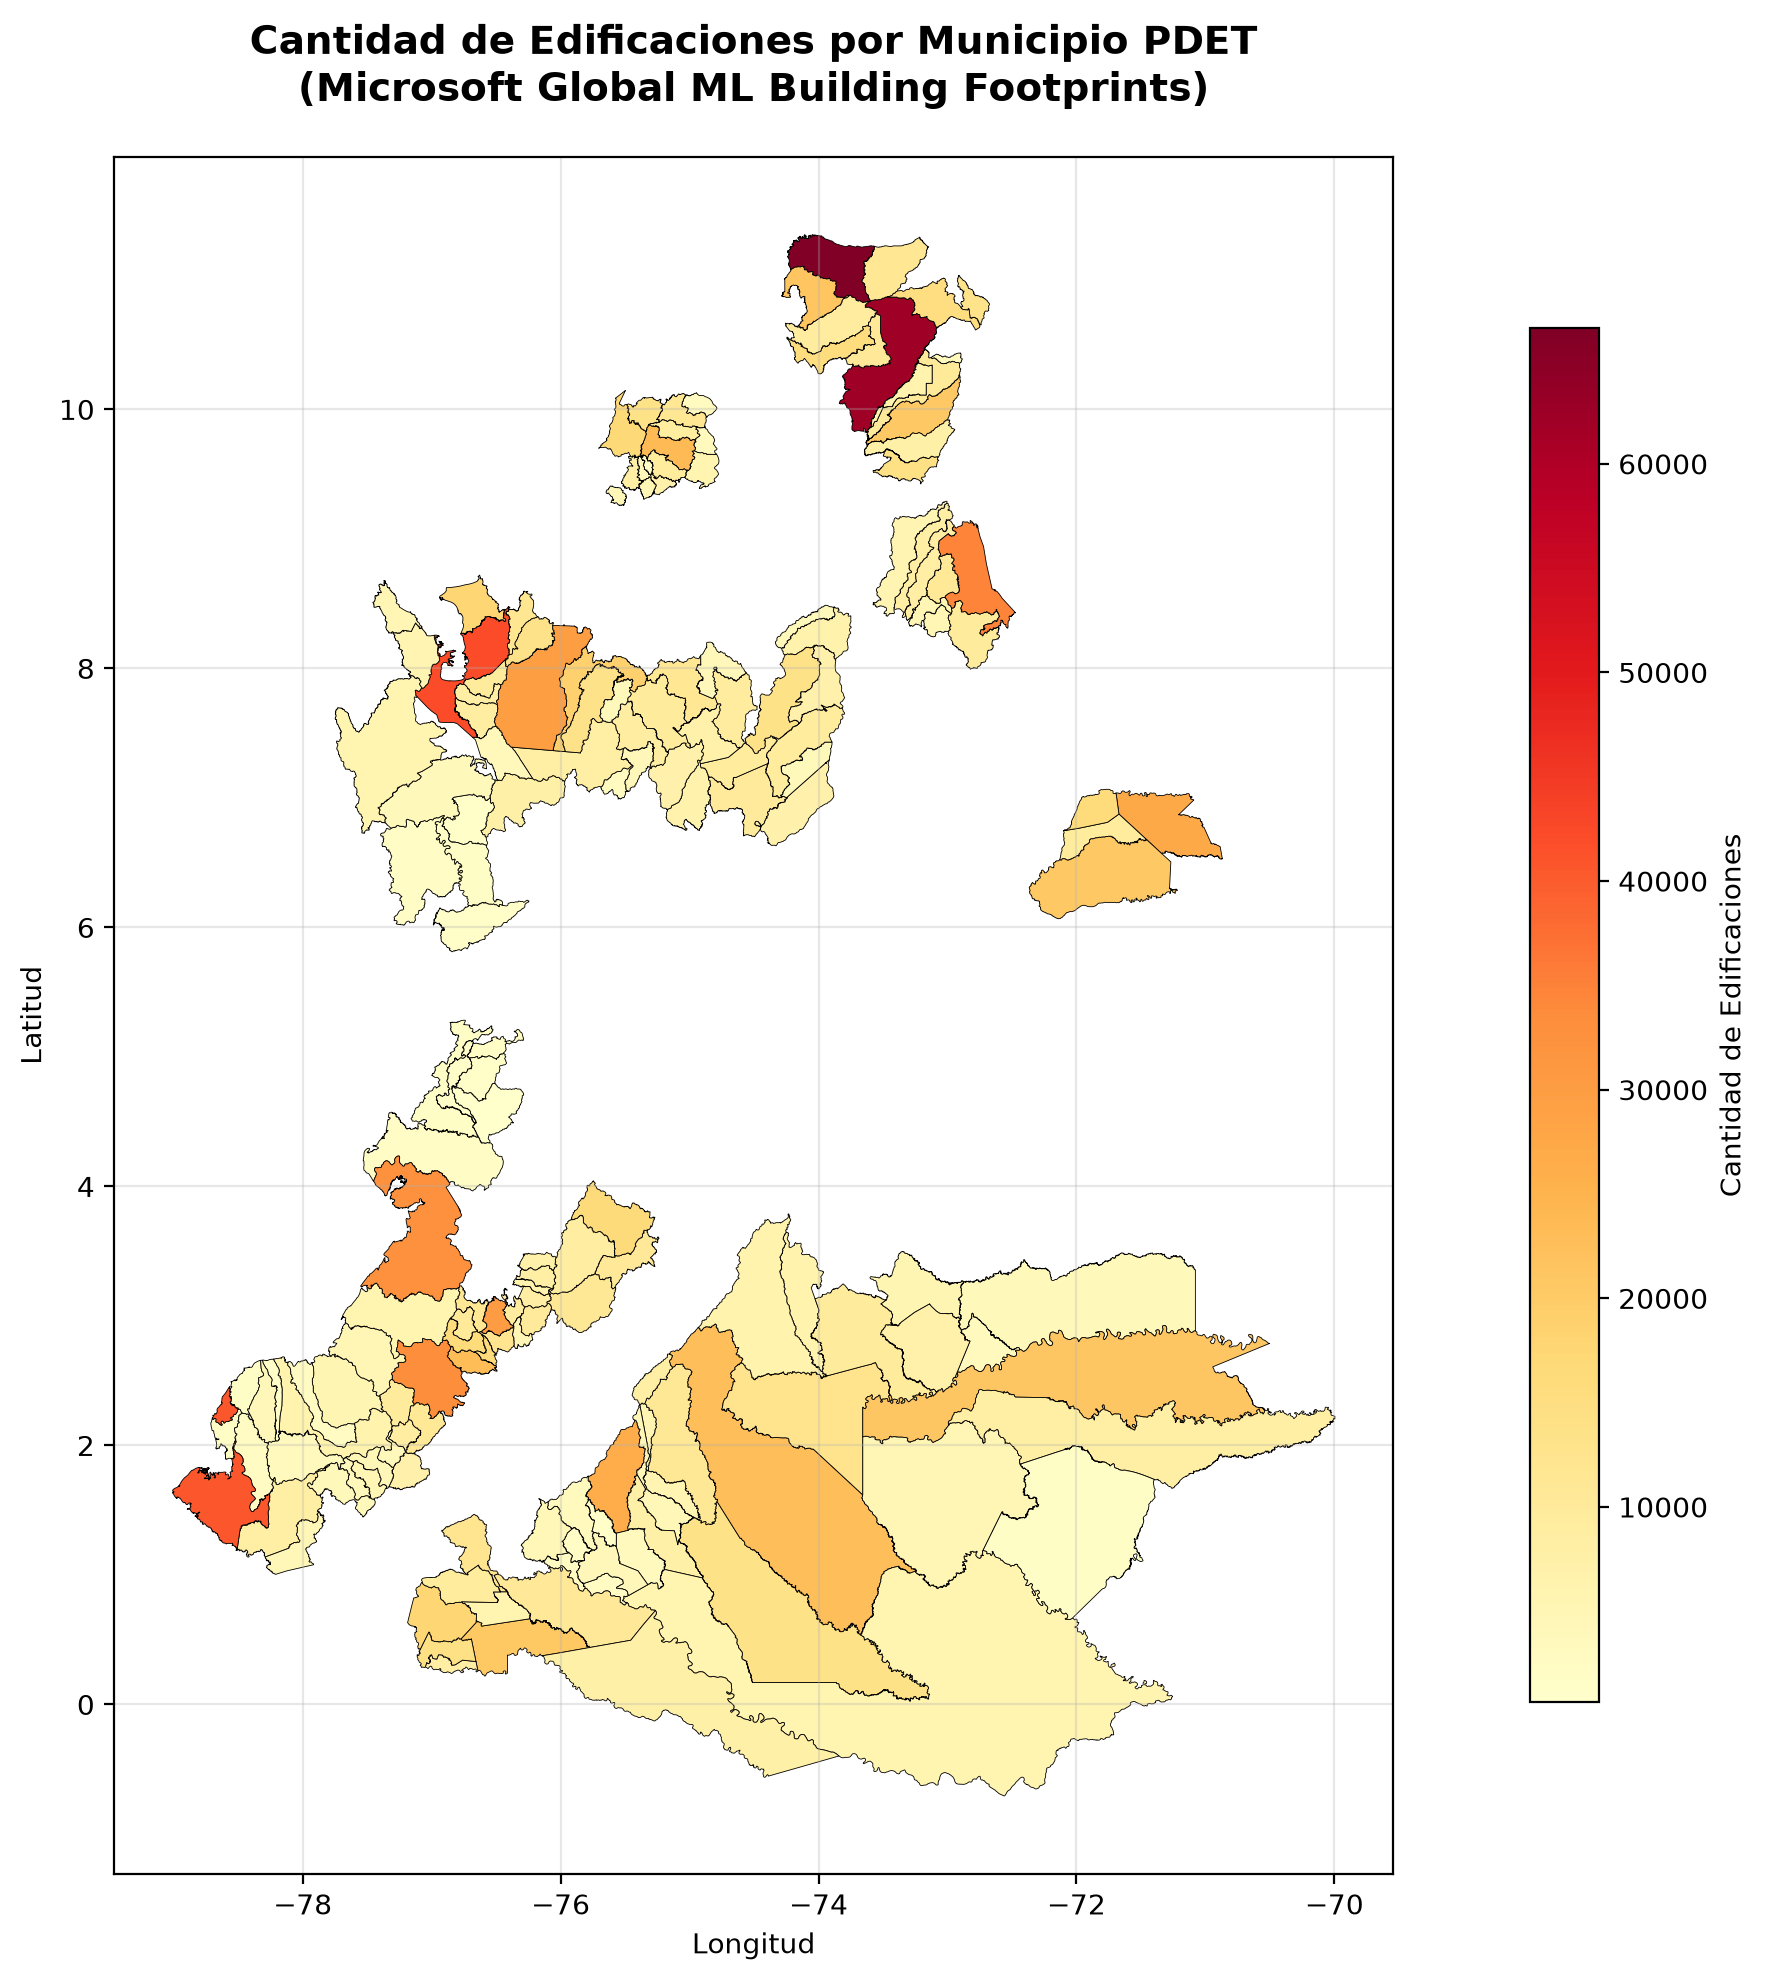
\includegraphics[width=0.95\textwidth]{figuras/map_buildings_count.png}
\caption{Distribución de cantidad de edificaciones por municipio. Las zonas con mayor concentración de población urbana (costa atlántica, ciudades intermedias) muestran mayores conteos.}
\label{fig:map_count}
\end{figure}

\subsection{Área Total de Techos}

\begin{figure}[h!]
\centering
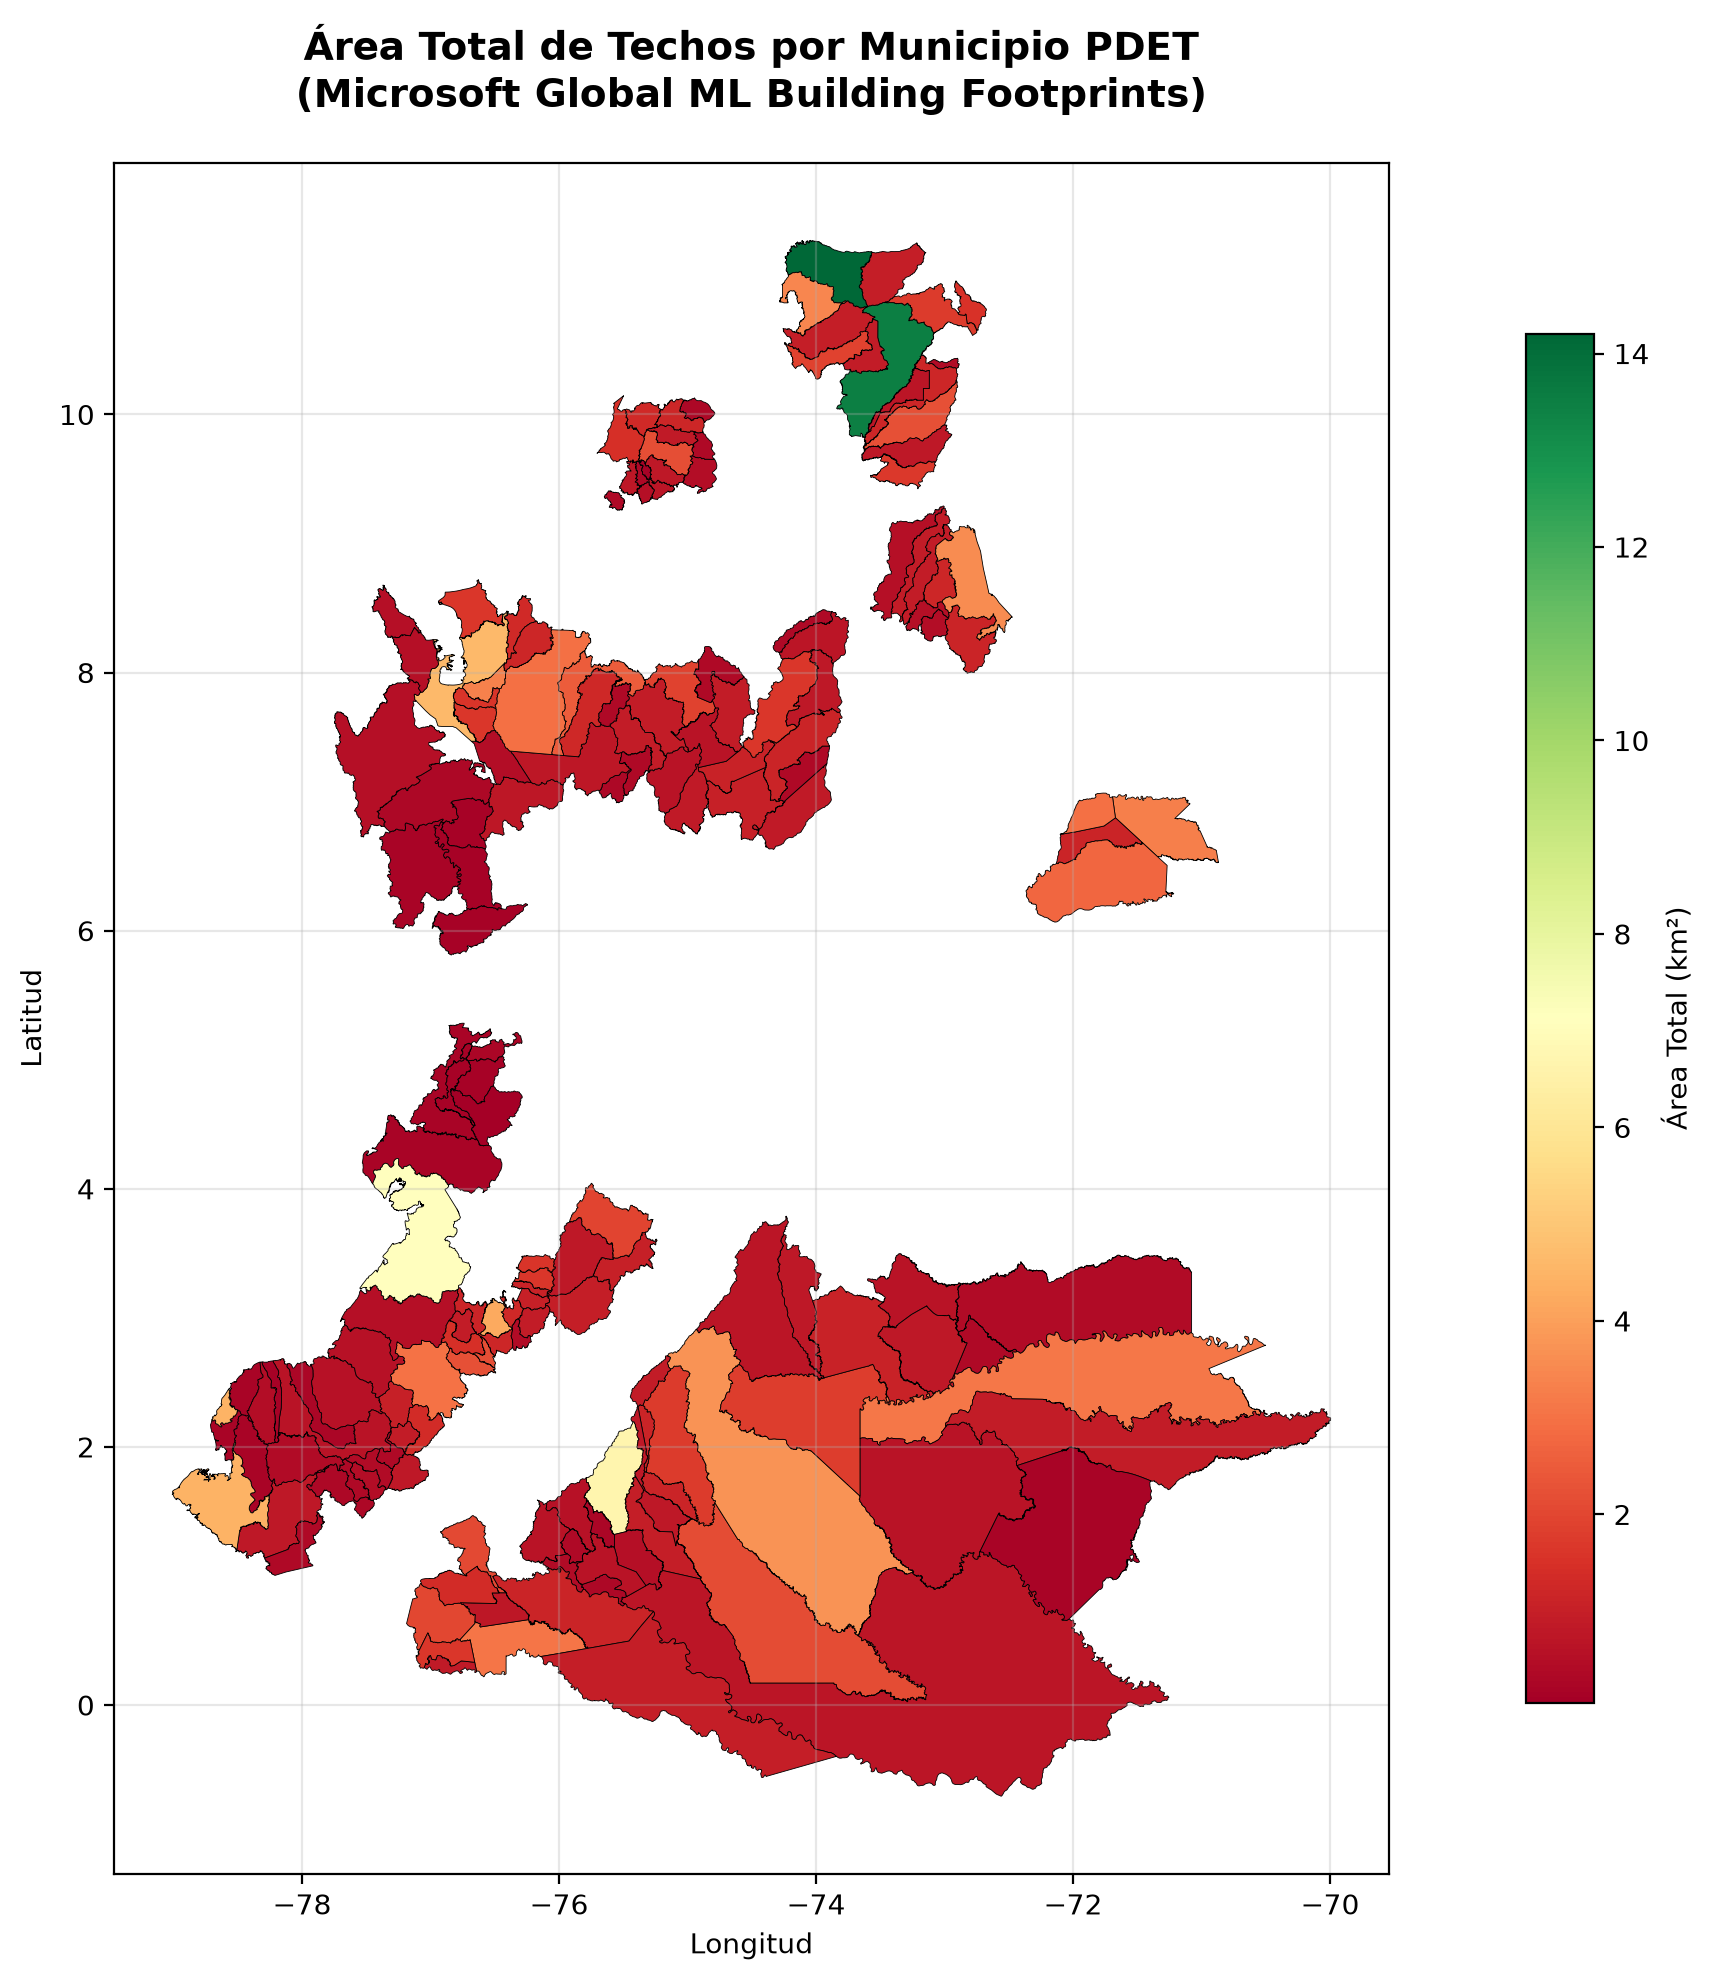
\includegraphics[width=0.95\textwidth]{figuras/map_total_area.png}
\caption{Distribución de área total de techos (km²) por municipio. Los municipios con más edificaciones no siempre tienen mayor área; esto refleja variaciones en el tamaño promedio de estructuras.}
\label{fig:map_area}
\end{figure}

\subsection{Área Media por Edificación}

\begin{figure}[h!]
\centering
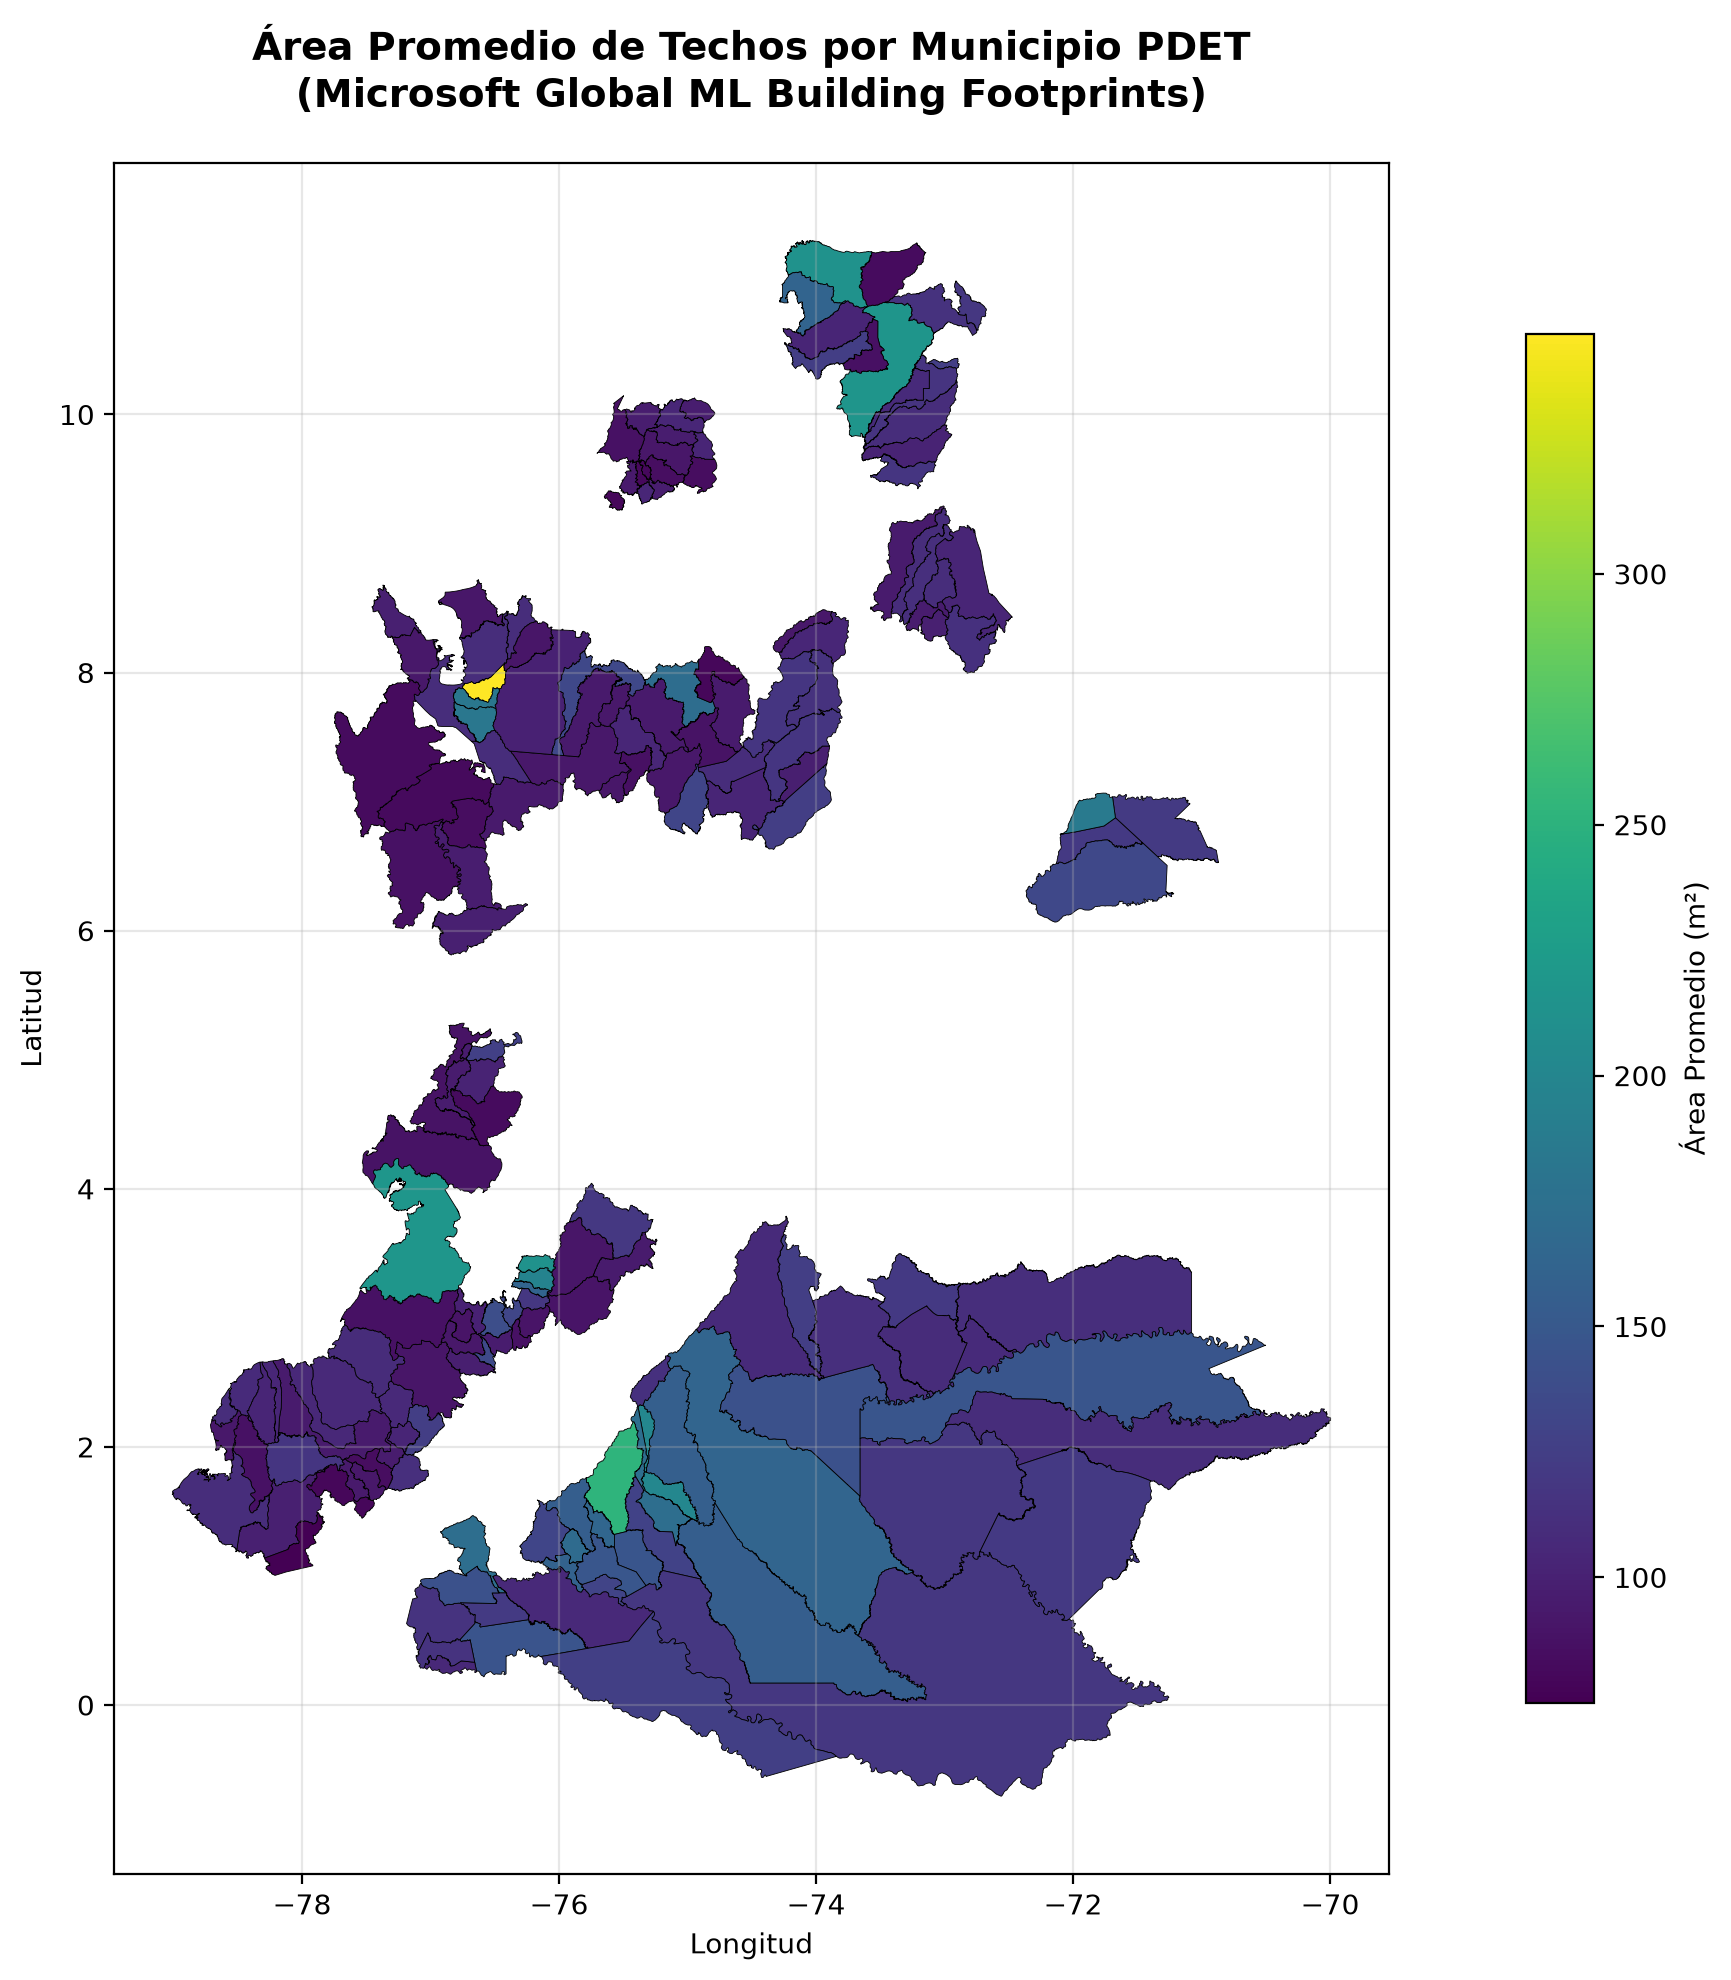
\includegraphics[width=0.95\textwidth]{figuras/map_mean_area.png}
\caption{Área promedio de cada edificación por municipio. Municipios con estructuras más grandes (bodegas, instalaciones industriales) muestran promedios más altos.}
\label{fig:map_mean}
\end{figure}

\newpage
\section{Municipios Destacados}

\subsection{Top 15 Municipios por Área de Techos}

\begin{table}[h!]
\small
\centering
\begin{tabular}{r|rp{3cm}p{3cm}r|r|r|r}
\toprule
\textbf{Rango} & \textbf{Código} & \textbf{Municipio} & \textbf{Subregión} & \textbf{Edif.} & \textbf{Área (km²)} & \textbf{Media (m²)} & \textbf{Med. (m²)} \\
\midrule
1 & 47001 & Santa Marta & Sierra Nevada - Perijá & 66.497 & 14,20 & 213,6 & 102,5 \\
2 & 20001 & Valledupar & Sierra Nevada - Perijá & 62.178 & 13,51 & 217,2 & 96,4 \\
3 & 76109 & Buenaventura & Pacífico Medio & 32.632 & 7,11 & 218,0 & 95,9 \\
4 & 18001 & Florencia & Cuenca del Caguán y Piedemonte Caqueteño & 26.487 & 6,68 & 252,1 & 108,1 \\
5 & 05837 & Turbo & Urabá Antioqueño & 42.084 & 4,63 & 109,9 & 74,1 \\
6 & 52835 & San Andrés de Tumaco & Pacífico y Frontera Nariñense & 40.707 & 4,47 & 109,9 & 77,3 \\
7 & 19698 & Santander de Quilichao & Alto Patía y Norte del Cauca & 30.341 & 4,22 & 139,0 & 93,2 \\
8 & 18753 & San Vicente del Caguán & Cuenca del Caguán y Piedemonte Caqueteño & 22.997 & 3,75 & 163,0 & 99,1 \\
9 & 54810 & Tibú & Catatumbo & 34.622 & 3,56 & 102,8 & 70,2 \\
10 & 47189 & Ciénaga & Sierra Nevada - Perijá & 21.475 & 3,47 & 161,5 & 92,0 \\
11 & 05045 & Apartadó & Urabá Antioqueño & 9.653 & 3,36 & 347,9 & 97,0 \\
12 & 81065 & Arauquita & Arauca & 27.178 & 3,31 & 121,7 & 82,4 \\
13 & 95001 & San José del Guaviare & Macarena - Guaviare & 21.020 & 3,10 & 147,3 & 87,9 \\
14 & 86568 & Puerto Asís & Putumayo & 20.868 & 3,04 & 145,8 & 87,1 \\
15 & 19256 & El Tambo & Alto Patía y Norte del Cauca & 33.433 & 3,03 & 90,5 & 69,8 \\
\bottomrule
\end{tabular}
\caption{Los 15 municipios con mayor área total de techos (Microsoft).}
\label{tab:top15}
\end{table}

\subsection{Bottom 15 Municipios por Área de Techos}

\begin{table}[h!]
\small
\centering
\begin{tabular}{r|rp{3cm}p{3cm}r|r|r|r}
\toprule
\textbf{Rango} & \textbf{Código} & \textbf{Municipio} & \textbf{Subregión} & \textbf{Edif.} & \textbf{Área (km²)} & \textbf{Media (m²)} & \textbf{Med. (m²)} \\
\midrule
170 & 27745 & Sipí & Chocó & 653 & 0,05 & 76,8 & 47,8 \\
169 & 27491 & Nóvita & Chocó & 1.403 & 0,11 & 78,5 & 54,6 \\
168 & 27450 & Medio San Juan & Chocó & 1.627 & 0,12 & 73,8 & 51,5 \\
167 & 05475 & Murindó [LOW] & Chocó & 1.311 & 0,13 & 99,2 & 70,0 \\
166 & 27425 & Medio Atrato & Chocó & 1.615 & 0,13 & 80,6 & 56,8 \\
165 & 27250 & El Litoral del San Juan & Chocó & 2.010 & 0,15 & 74,6 & 52,0 \\
164 & 27205 & Condoto & Chocó & 2.110 & 0,16 & 75,8 & 50,8 \\
163 & 27150 & Carmen del Darién & Chocó & 3.832 & 0,30 & 78,3 & 54,5 \\
162 & 27099 & Bojayá & Chocó & 2.004 & 0,16 & 79,8 & 55,0 \\
161 & 05873 & Vigía del Fuerte [LOW] & Chocó & 1.714 & 0,17 & 99,1 & 68,2 \\
160 & 73616 & Rioblanco & Sur del Tolima & 9.018 & 0,51 & 56,6 & 41,4 \\
159 & 52621 & Roberto Payán & Pacífico y Frontera Nariñense & 2.501 & 0,20 & 80,0 & 54,1 \\
158 & 52612 & Ricaurte & Pacífico y Frontera Nariñense & 4.878 & 0,41 & 84,0 & 56,4 \\
157 & 19418 & López de Micay [LOW] & Pacífico Medio & 5.968 & 0,47 & 78,8 & 54,5 \\
156 & 27615 & Riosucio & Chocó & 6.107 & 0,49 & 80,3 & 55,5 \\
\bottomrule
\end{tabular}
\caption{Los 15 municipios con menor área total de techos (Microsoft). [LOW] indica cobertura insuficiente de Google.}
\label{tab:bottom15}
\end{table}

\newpage
\section{Análisis por Subregión PDET}

\subsection{Tabla de Totales por Subregión}

\begin{table}[h!]
\small
\centering
\begin{tabular}{lrr|r}
\toprule
\textbf{Subregión PDET} & \textbf{Edificaciones} & \textbf{Área (km²)} & \textbf{Municipios} \\
\midrule
Sierra Nevada - Perijá & 287.899 & 46,20 & 20 \\
Alto Patía y Norte del Cauca & 265.317 & 30,17 & 15 \\
Cuenca del Caguán y Piedemonte Caqueteño & 131.224 & 22,52 & 7 \\
Urabá Antioqueño & 110.379 & 15,25 & 6 \\
Putumayo & 106.390 & 13,79 & 11 \\
Montes de María & 126.814 & 11,78 & 10 \\
Macarena - Guaviare & 91.513 & 11,46 & 8 \\
Bajo Cauca y Nordeste Antioqueño & 99.599 & 10,65 & 10 \\
Arauca & 73.091 & 10,18 & 4 \\
Catatumbo & 87.522 & 9,20 & 6 \\
Pacífico Medio & 48.837 & 8,74 & 7 \\
Sur de Córdoba & 79.095 & 8,30 & 8 \\
Pacífico y Frontera Nariñense & 77.821 & 8,09 & 5 \\
Sur de Bolívar & 51.577 & 5,82 & 7 \\
Sur del Tolima & 46.767 & 4,74 & 5 \\
Chocó & 36.690 & 3,40 & 10 \\
\midrule
\textbf{TOTAL PDET} & \textbf{1.720.535} & \textbf{220,27} & \textbf{170} \\
\bottomrule
\end{tabular}
\caption{Agregaciones de edificaciones y área de techos por subregión PDET.}
\label{tab:subregions}
\end{table}

\subsection{Gráfica: Comparativa de Subregiones}

\begin{figure}[h!]
\centering
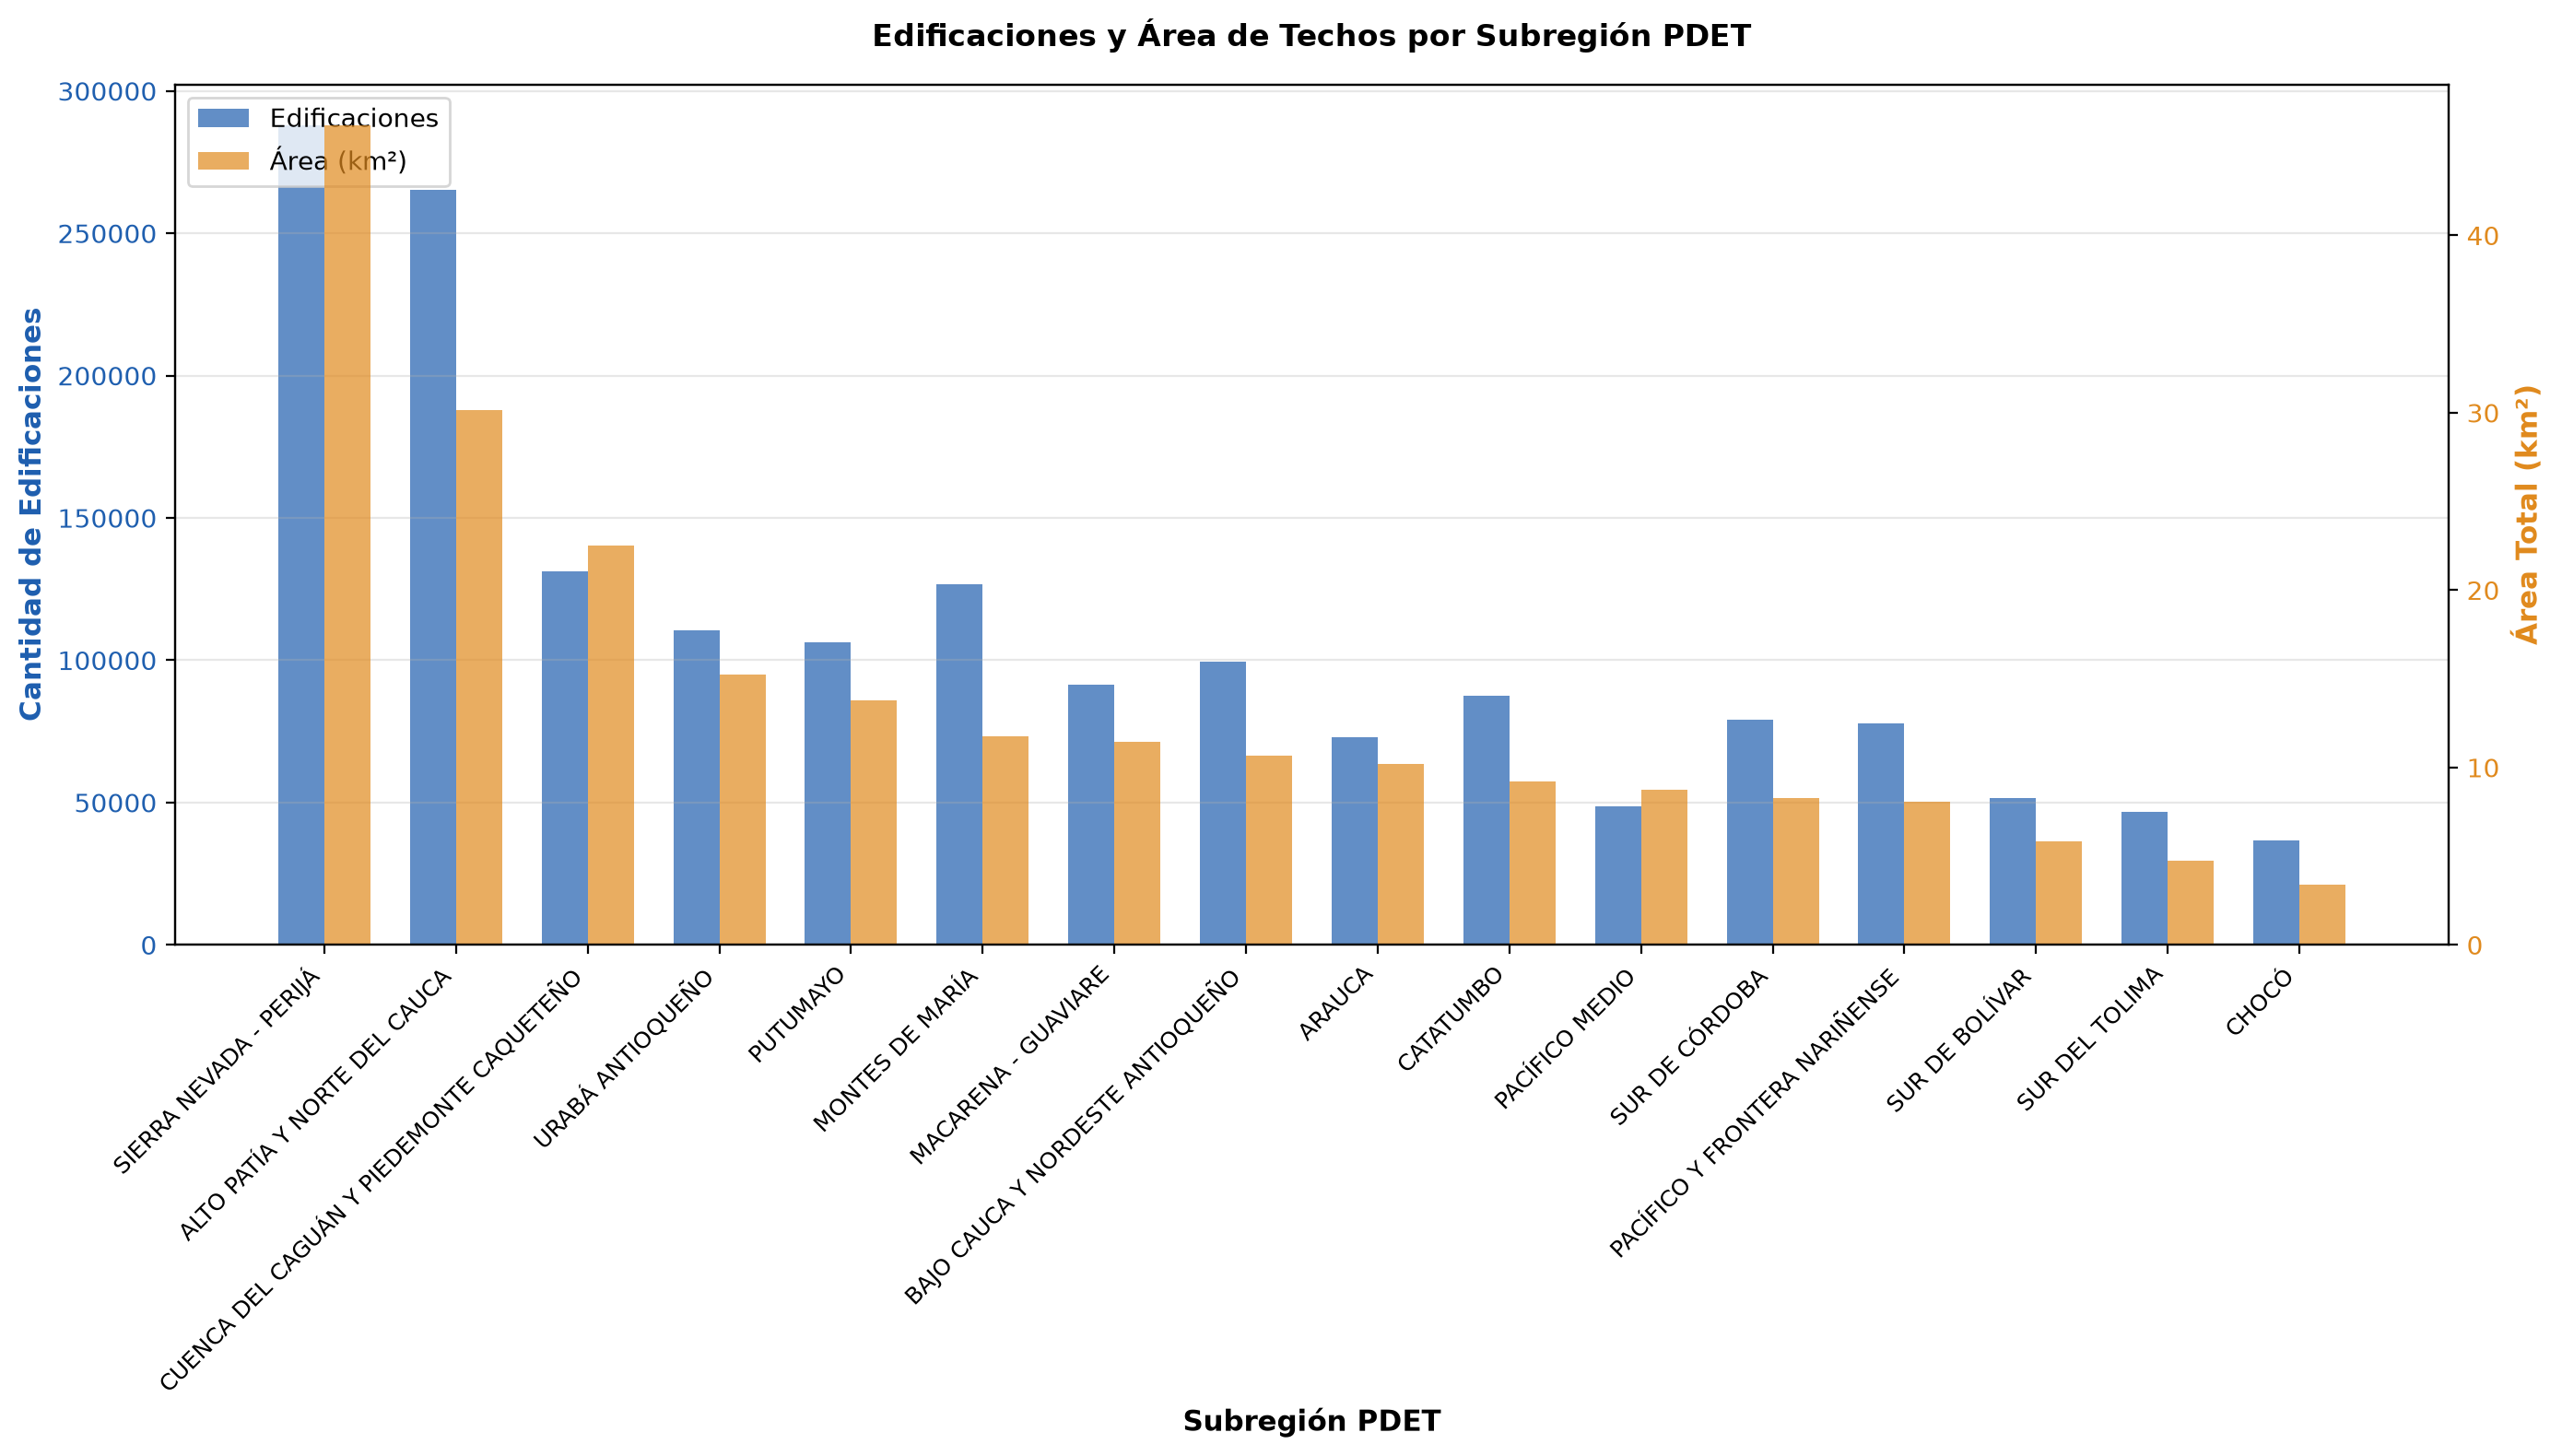
\includegraphics[width=0.95\textwidth]{figuras/subregion_totals.png}
\caption{Comparativa de cantidad de edificaciones (barras azules) y área total (barras naranjas) por subregión. Sierra Nevada - Perijá y Alto Patía dominan en ambas métricas.}
\label{fig:subregions}
\end{figure}

\newpage
\section{Gráficos Comparativos}

\subsection{Top 15 Municipios}

\begin{figure}[h!]
\centering
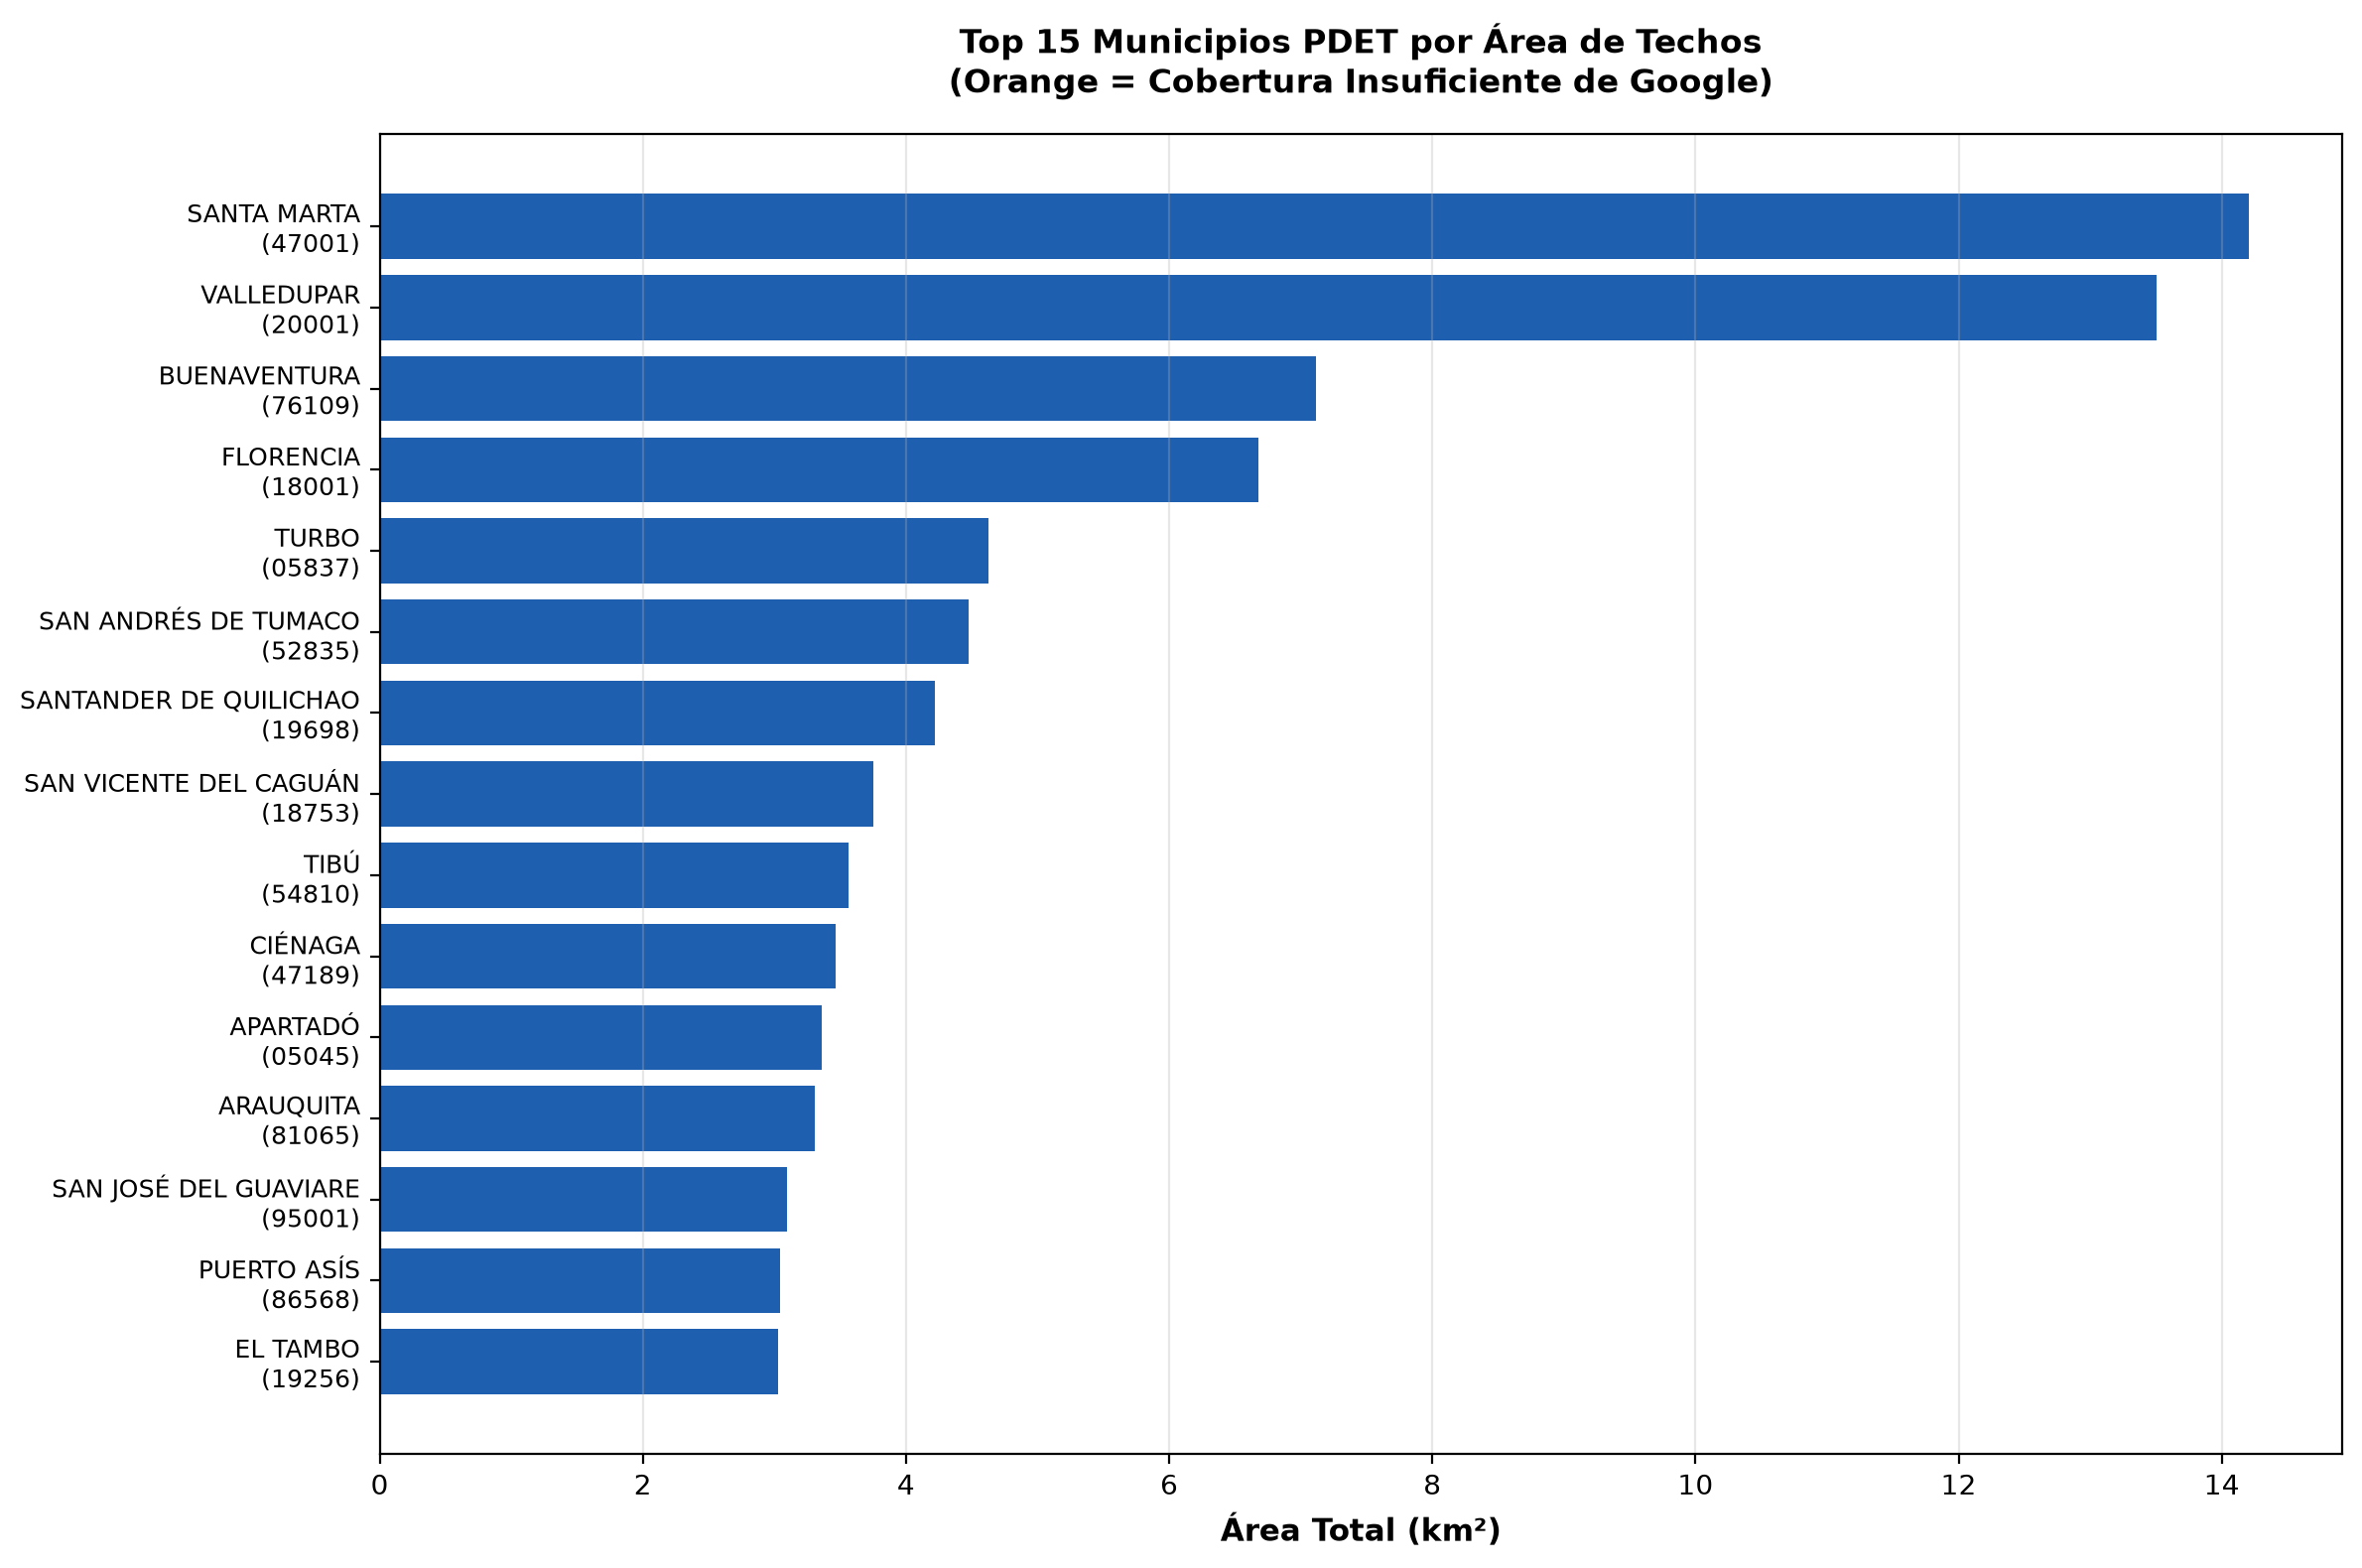
\includegraphics[width=0.9\textwidth]{figuras/bar_top_municipalities.png}
\caption{Área total de techos en los 15 municipios con mayor valor. Las barras naranjas indican municipios con cobertura insuficiente de Google.}
\label{fig:bar_top}
\end{figure}

\subsection{Correlación: Cantidad vs Área}

\begin{figure}[h!]
\centering
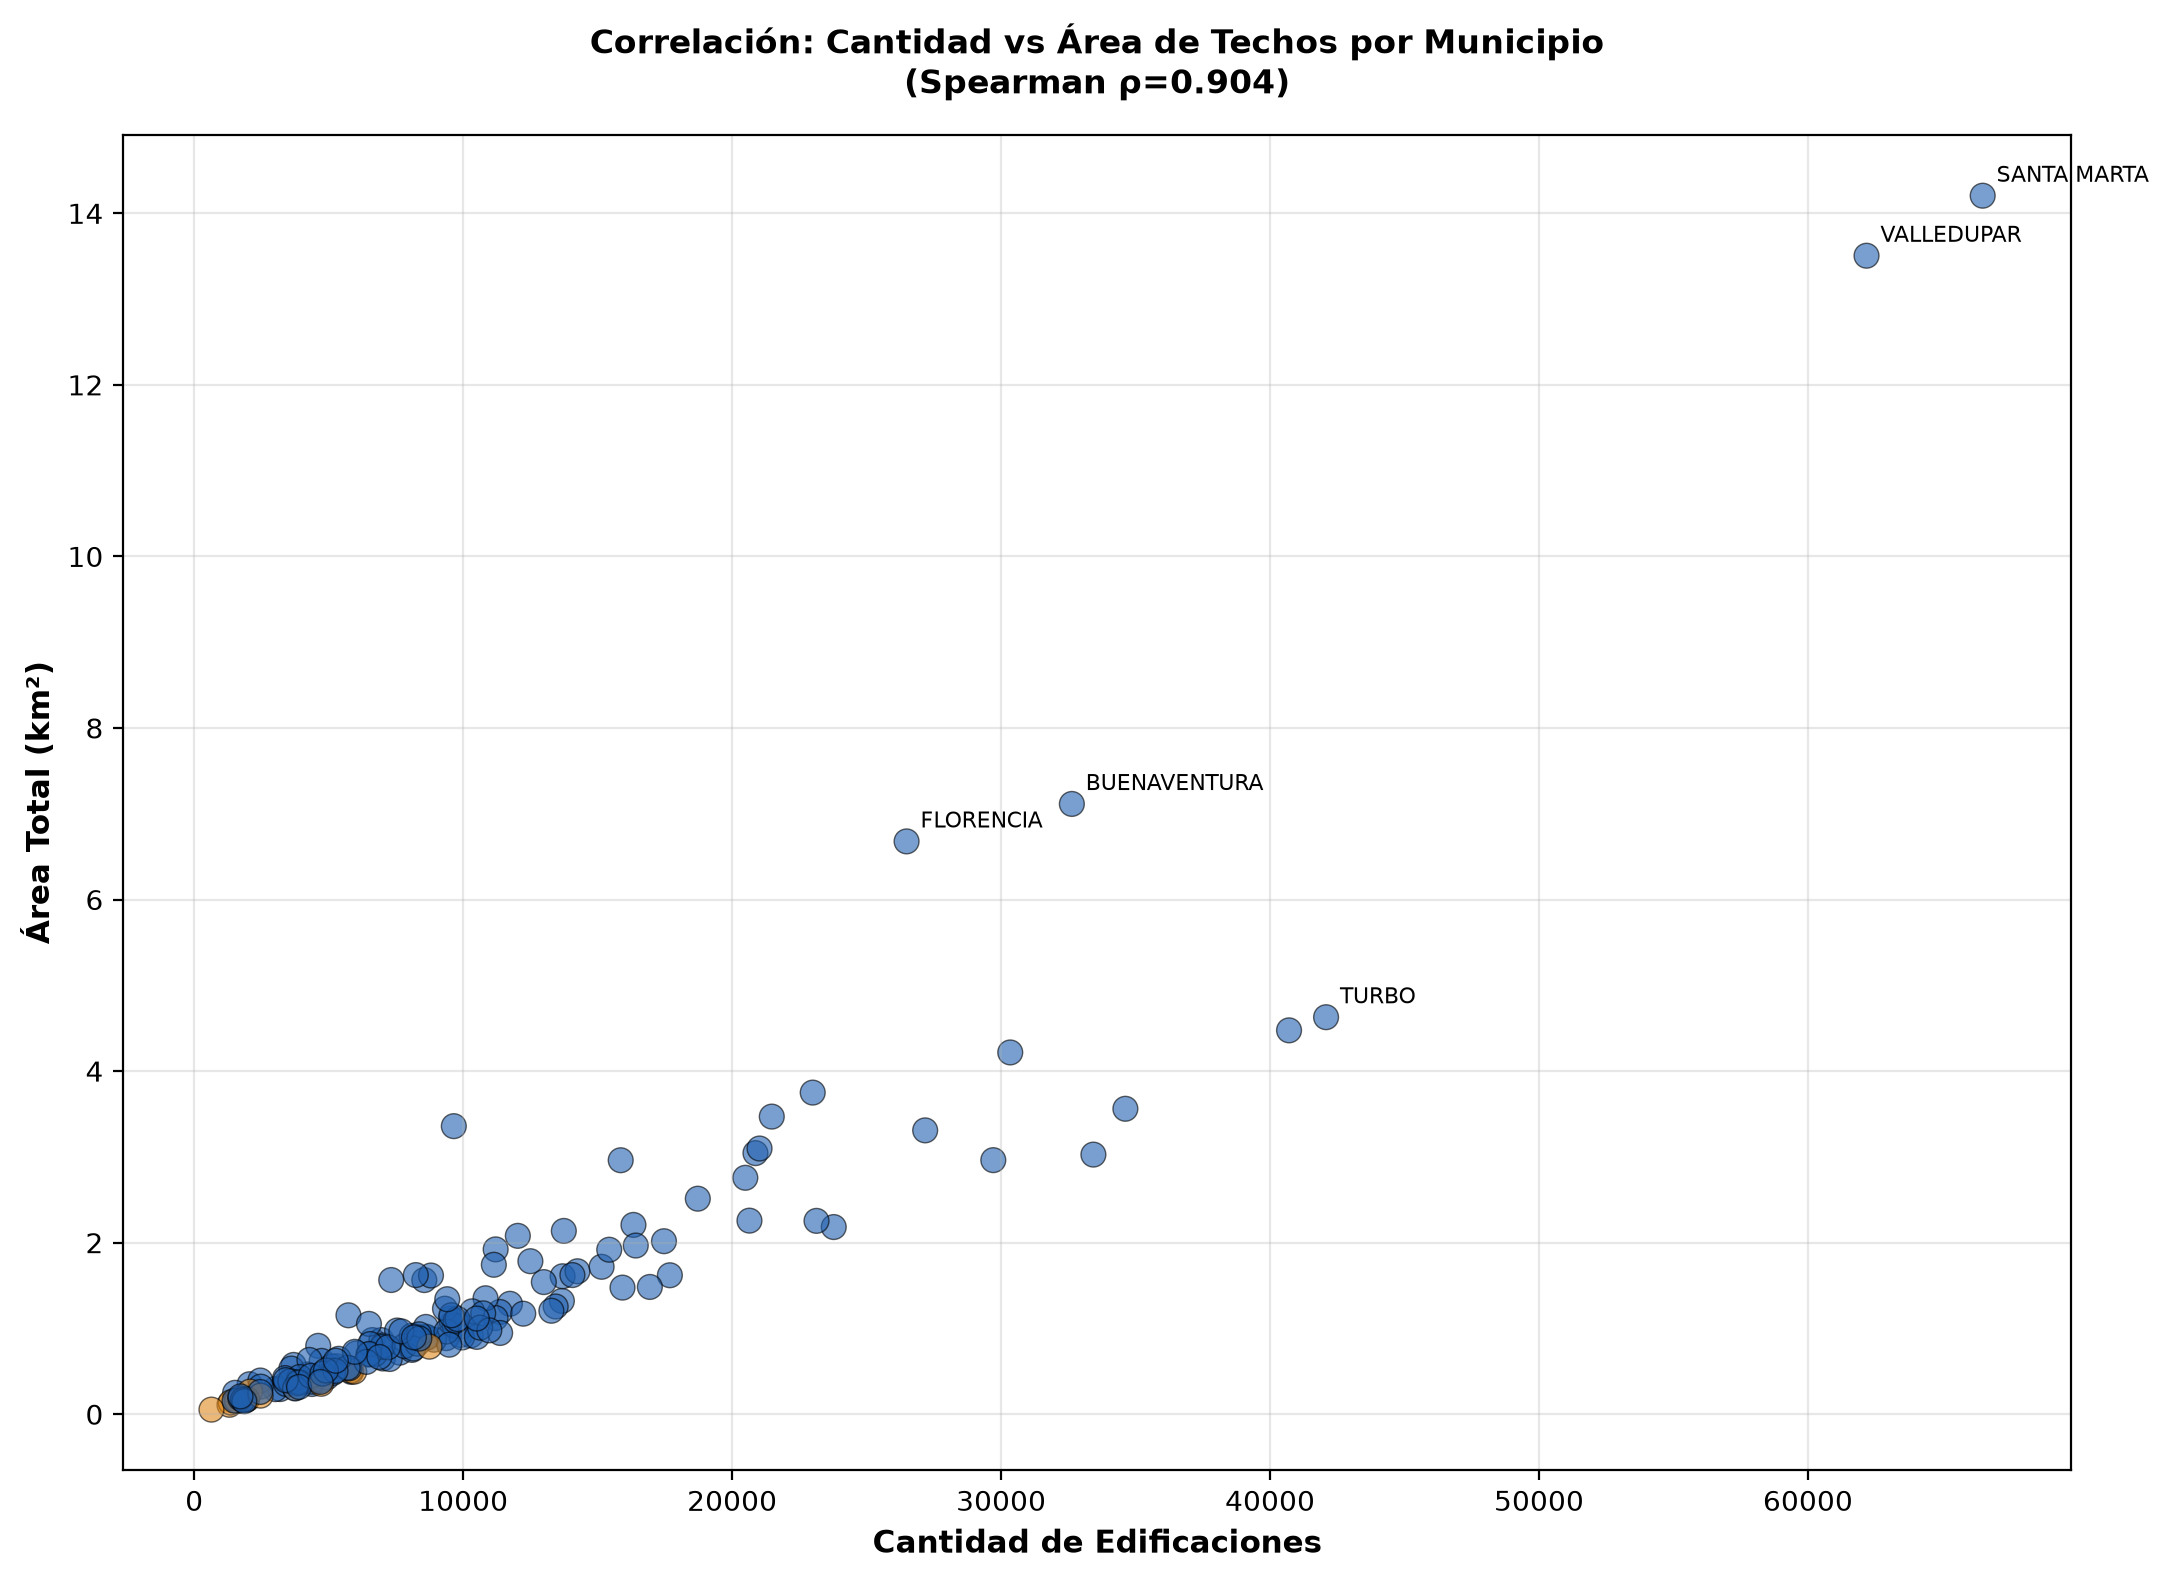
\includegraphics[width=0.9\textwidth]{figuras/scatter_count_vs_area.png}
\caption{Scatter plot de cantidad de edificaciones vs área total (km²) por municipio. Correlación Spearman r = 0,904 (muy fuerte). Cada punto es un municipio; puntos naranjas tienen cobertura insuficiente de Google.}
\label{fig:scatter}
\end{figure}

\newpage
\section{Comparación Microsoft vs Google}

\subsection{Hallazgos Clave}

\begin{itemize}
    \item \textbf{Cobertura espacial:} Microsoft: 170 municipios PDET. Google: 165 municipios.
    \item \textbf{Conteo de edificaciones:} Microsoft 1.720.535 incluidas; Google 1,53× (aproximadamente 2.634.000).
    \item \textbf{Área total:} Microsoft 220,27 km²; Google 1,005× (221,37 km²). Prácticamente idéntica.
    \item \textbf{Correlación Spearman (edificaciones):} 0,904 (fuerte concordancia en ranking de municipios).
    \item \textbf{Correlación Spearman (área):} 0,938 (muy fuerte concordancia en ranking de área).
\end{itemize}

\subsection{Municipios con Cobertura Insuficiente de Google}

Los siguientes 15 municipios tienen menos del 20\% de las edificaciones detectadas por Google respecto a Microsoft. No se recomienda comparación directa en estos casos:

\begin{table}[h!]
\small
\centering
\begin{tabular}{rp{3cm}p{3cm}r}
\toprule
\textbf{Código} & \textbf{Municipio} & \textbf{Subregión} & \textbf{MS Edif.} \\
\midrule
05475 & Murindó & Chocó & 1.311 \\
05873 & Vigía del Fuerte & Chocó & 1.714 \\
19418 & López de Micay & Pacífico Medio & 5.968 \\
27099 & Bojayá & Chocó & 2.004 \\
27150 & Carmen del Darién & Chocó & 3.832 \\
27205 & Condoto & Chocó & 2.110 \\
27250 & El Litoral del San Juan & Chocó & 2.010 \\
27425 & Medio Atrato & Chocó & 1.615 \\
27450 & Medio San Juan & Chocó & 1.627 \\
27491 & Nóvita & Chocó & 1.403 \\
27615 & Riosucio & Chocó & 6.107 \\
27745 & Sipí & Chocó & 653 \\
52612 & Ricaurte & Pacífico y Frontera Nariñense & 4.878 \\
52621 & Roberto Payán & Pacífico y Frontera Nariñense & 2.501 \\
73616 & Rioblanco & Sur del Tolima & 9.018 \\
\bottomrule
\end{tabular}
\caption{Municipios con cobertura insuficiente en Google (< 20\% de edificaciones respecto a Microsoft).}
\label{tab:lowcov}
\end{table}

\section{Limitaciones y Consideraciones}

\begin{itemize}
    \item \textbf{Huellas muy grandes:} En Microsoft, el percentil 99 del área es 912 m² y el máximo 44.720 m². Son bodegas e instalaciones que sí representan techo real, pero pueden no ser aprovechables para energía solar.

    \item \textbf{Área aprovechable vs huella:} La cifra reportada es la proyección geodésica del edificio (huella en m²). Para obtener área aprovechable, se debe aplicar un factor de utilización que considere orientación, sombra, pendiente y orientación de paneles (típicamente 30\%--60\% de la huella total).

    \item \textbf{Cobertura de Google:} 15 municipios tienen representación deficiente en Google. Las causas no han sido verificadas y pueden incluir nubosidad, resolución de imagen, o deforestación.

    \item \textbf{Calidad de geometrías municipales:} Las geometrías de PDET provienen del MGN2025 del DANE. Cambios administrativos posteriores a esta fecha no están reflejados.

    \item \textbf{Fecha de acceso:} Microsoft Building Footprints v2026-02-03, accedida 13 de noviembre de 2026. Futuras versiones pueden cambiar resultados.
\end{itemize}

\section{Reproducibilidad}

Para reproducir este análisis desde cero:

\begin{enumerate}
    \item Asegurarse de que MongoDB está disponible y la base \texttt{upme\_pdet} contiene las colecciones \texttt{buildings} y \texttt{municipalities} cargadas según Entrega 3.
    \item Ejecutar desde la raíz del proyecto:
    \begin{verbatim}
    bash scripts/run_entrega4_pipeline.sh
    \end{verbatim}
    \item El script ejecutará secuencialmente:
    \begin{verbatim}
    python scripts/07_entrega4_analysis.py
    python scripts/08_entrega4_visualizations.py
    python scripts/09_entrega4_tables.py
    cd docs/delivery4 && latexmk -pdf entrega4_informe.tex
    \end{verbatim}
    \item El PDF final se genera en \texttt{docs/delivery4/Entrega4\_Analisis\_Techos.pdf}.
\end{enumerate}

Todos los pasos son automatizados: no hay transcripción manual de cifras. Los números que aparecen en este informe se leen directamente desde los archivos de entrada (CSV, JSON) mediante scripts de Python.

\newpage
\section*{Anexo: Archivos de Entrada y Salida}

\textbf{Entrada:}
\begin{itemize}
    \item \texttt{outputs/rooftop\_stats\_ms.csv} — 170 municipios con conteo y áreas
    \item \texttt{outputs/eda/eda\_buildings\_summary.json} — Comparativa MS vs Google y metadatos
    \item \texttt{data/processed/municipalities.geojsonl} — Geometrías 170 municipios PDET
\end{itemize}

\textbf{Salida (generada automáticamente):}
\begin{itemize}
    \item \texttt{outputs/entrega4\_analysis\_summary.json} — JSON unificado con todos los datos
    \item \texttt{docs/delivery4/figuras/*.png} — 6 mapas y gráficos (200 dpi)
    \item \texttt{docs/delivery4/entrega4\_analysis\_tables.md} — Tablas en markdown
    \item \texttt{docs/delivery4/Entrega4\_Analisis\_Techos.pdf} — Este informe compilado
\end{itemize}

\vspace{2cm}
\hrule
\vspace{0.5cm}
\textit{Informe generado automáticamente el \today. Acceso a código fuente: \texttt{github.com/dba-upme-pdet/techos-solares-pdet}}

\end{document}
